% kenkyukai_template.tex を編集

%\documentstyle[epsf,twocolumn]{jarticle}       %LaTeX2.09仕様
\documentclass[twocolumn]{jarticle}
%%%%%%%%%%%%%%%%%%%%%%%%%%%%%%%%%%%%%%%%%%%%%%%%%%%%%%%%%%%%%%
%%
%%  基本 バージョン
%%
%%%%%%%%%%%%%%%%%%%%%%%%%%%%%%%%%%%%%%%%%%%%%%%%%%%%%%%%%%%%%%%%
\setlength{\topmargin}{-45pt}
%\setlength{\oddsidemargin}{0cm}
\setlength{\oddsidemargin}{-7.5mm}
%\setlength{\evensidemargin}{0cm}
\setlength{\textheight}{24.1cm}
%setlength{\textheight}{25cm}
\setlength{\textwidth}{17.4cm}
%\setlength{\textwidth}{172mm}
\setlength{\columnsep}{11mm}


%【節がかわるごとに(1.1)(1.2) …(2.1)(2.2)と数式番号をつけるとき】
%\makeatletter
%\renewcommand{\theequation}{%
%\thesection.\arabic{equation}} %\@addtoreset{equation}{section}
%\makeatother

%\renewcommand{\arraystretch}{0.95} 行間の設定

%%%%%%%%%%%%%%%%%%%%%%%%%%%%%%%%%%%%%%%%%%%%%%%%%%%%%%%%
\usepackage[dvipdfm]{graphicx}   %pLaTeX2e仕様(要\documentstyle ->\documentclass)
%%%%%%%%%%%%%%%%%%%%%%%%%%%%%%%%%%%%%%%%%%%%%%%%%%%%%%%%

% 図を別のフォルダから読み込む
\graphicspath{{./figure/}}



\begin{document}

\twocolumn[
\noindent

\hspace{1em}

情報工学実験I\hspace{-.1em}I
\hfill
\ \ B3 多田 瑞葵


\vspace{2mm}

\hrule

\begin{center}
{\Large \bf BERT を用いた深層言語処理における品詞推定の調査}
\end{center}


\hrule
\vspace{3mm}
]

\section{はじめに}
近年,人工知能や深層学習による創作に関する研究が盛んになっている.自然言語処理の分野においても小説の生成を目指した文や文章の生成などが研究されているが,これには画像などの生成とは異なる課題がある.その一つが,生成される文の文法情報や品詞情報が正しく得られるかどうかという課題である.文を生成するには言葉を正しくならべる必要があり,それには正しい文法や品詞の理解が欠かせない.\par
本実験では,最近注目を集めている深層言語モデル BERT を用いて,文生成の基礎である文の品詞の情報がどの程度獲得できているかを実験をもとに調査した.


\section{要素技術}
% 要素技術と従来手法をあわせて要素技術

  \subsection{BERT}
BERT (Bidirectional Encoder Representations from Transformers)\cite{DBLP} は,2018 年 10 月に Google の Jacob Devlin らが発表した,Transformer による双方向のエンコーダーを用いた言語モデルである.文の入力に対して,入力された文および,文に含まれる各単語に対応する分散表現を出力する.従来の言語モデルは特定の自然言語処理タスクにのみ対応しており,タスクに応じてモデルの修正が必要であった.しかし BERT はファインチューニングをすることで,モデルの修正をせずに様々なタスクに応用でき,汎化性に優れている.また当時 11 個のタスクに対して state-of-the-art を達成しており精度が高い.\par
BERT は事前学習モデルであり,入力文の一部の単語を "[MASK]" 記号に置き換えてその元単語を予測する「masked language model」に基づいたタスクと,2 つの入力文に対して文の連続性を識別する「next sentence prediction」のタスクによって学習する.\par
本実験では,東北大学から公開されている,日本語 Wikipedia の文章を用いて事前学習されたモデル\footnote{https://www.nlp.ecei.tohoku.ac.jp/news-release/3284/}を使用した.このモデルでは,入力文を MeCab\footnote{https://taku910.github.io/mecab/} により形態素解析し,WordPiece という手法により subword 化している.


  % BERT は一部の単語を [MASK] に置き換えることで,そこの単語を予測してくれます.そもそも BERT は二種類の事前学習をしていて,単語の予測と文の関係性の予測の二つを勉強していて,それによってとても賢いです.今回はその単語の予測の部分(BERT で事前学習している部分)を使うのですが,事前学習とタスクが同じなので,ファインチューニングが不要ですか...?(何もわかっていない顔)


% 脚注の入れ方
%http://www.latex-cmd.com/struct/footnote.html

  %
  % \subsection{MeCab}
  % MeCabは,オープンソース形態素解析エンジンであり,京都大学情報学研究科-日本電信電話株式会社コミュニケーション科学基礎研究所共同研究ユニットプロジェクトを通して開発された.
  % \par
  % 日本語は,文中で単語が区切りなく並べられているため,BERT を使う前に文を単語に区切る必要がある.書くことがない!!!!!!!!!!
  %
  % 東北大学から公開されている BERT の日本語モデルは,形態素解析器に MeCab を用いて事前学習している.そのため本実験でも形態素解析に MeCab を用いた.
  % (HPに書いてあったのをそのまま書いただけで,しかもこの〜〜プロジェクトのリンクが切れてるのでまたちゃんと調べておく)

  % また,形態素解析器はたくさんあるのだけれど,本実験で使用する BERT は MeCab を用いたトークナイズ(=形態素解析?)によって訓練されているため,同様に MeCab を使用する.



\section{使用データセット}
本実験では,叙述的な文を対象に品詞を推定するため,毎日新聞データセット\footnote{https://www.nichigai.co.jp/sales/mainichi/mainichi-data.html}の新聞記事を用いた.2008 年の 1 面に掲載された記事の中から文として成立しているものを抜き出し,それぞれの文章に対して "□","×" などの記号,"<>" などの間に書かれた注釈等を取り除いた.
 



%\section{実験手法}
% 従来手法があるなら提案手法とする

\section{数値実験}
  \subsection{実験の前処理}
本実験では,文中の単語を "[MASK]" 記号に置き換え,元単語が各品詞(名詞,動詞,形容詞)であるかどうかを正しく出力できるかを調査した.\par
前処理として,データセットの各文に対して分かち書きをし,単語に分割した.一文の単語の中から 1 つをランダムに選択して "[MASK]" 記号に置き換えた.置き換えた箇所の元単語が名詞である文にラベル 1 を,そうでない文にラベル 0 を付与し,実験に用いるデータとした.また,置き換えた箇所の元単語が動詞である文にラベル 1 を,そうでない文にラベル 0 を付与し直し,実験に用いるデータとした.同様に,形容詞についてもラベルを付与し直して実験に用いるデータとした.以上の手順で名詞,動詞,形容詞の推定用のデータセットをそれぞれ 1 つずつ用意した.\par

  \subsection{実験}
まず,データセットの各文に対して,データの偏りによる精度の差を避けるため,ラベル 0 とラベル 1 のデータ数を同じ 5000 個に揃えた.この各文を BERT に入力して,得られた各単語の分散表現を多層パーセプトロン(MLP)に入力して分類した.表 \ref{tb:1} に本実験で用いた MLP のパラメータを示す.学習率は,BERT の初出論文 \cite{DBLP} で推薦されている値を使用した.また,データ数が少ないため,訓練データに対して 5 分割交差検証による平均値を確認して評価した.


\begin{table}[t]
	\caption{実験で用いた MLP のパラメータ}
  \begin{center}
  \begin{tabular}{|c|c|} \hline
  パラメータ & 値  \\ \hline \hline
  入力層の次元数	& 分散表現の次元数 \\ %\cline{2-2}
  隠れ層の次元数	& 768 \\
  出力層の次元数	& 2 \\
  エポック数 & 10 \\
  バッチサイズ & 10 \\
  損失関数 & cross entropy \\
  最適化関数 & Adam \\
  学習率 & $5\times10^{-5}$ \\ \hline
	\end{tabular}
  \end{center}
	\label{tb:1}
\end{table}




\subsection{実験結果}

図 \ref{fig:mei_acc} に,学習時の accuracy と loss の推移を示す.横軸はどちらも epoch 数を,縦軸はそれぞれ accuraacy と loss を表している.
% ここに学習の図の感想を書く
% 過学習してるとか,正常に学習してるとか
表 \ref{tb:2} に品詞の推定結果を示す.



% \begin{minipage}{0.5\hsize} で,図を横並びに挿入できる
\begin{figure}[tbp]
      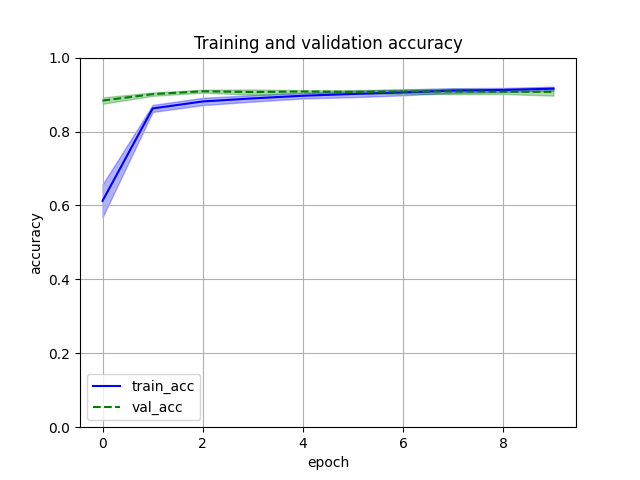
\includegraphics[width=\linewidth]{meishi_acc.png}
      \caption{名詞推定時の accuracy の推移}
      \label{fig:mei_acc}
\end{figure}
\begin{figure}[tbp]
      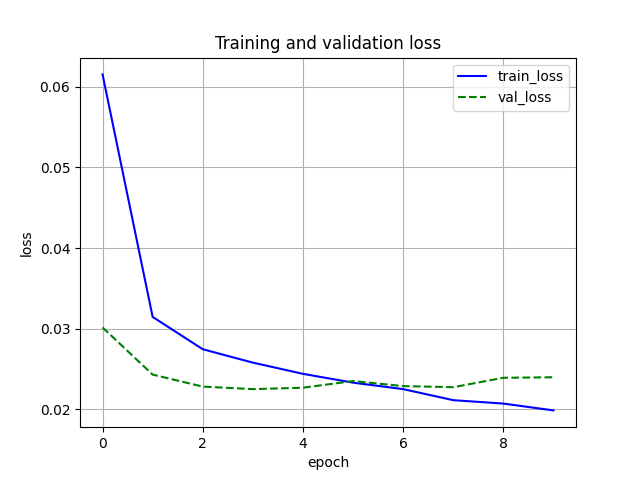
\includegraphics[width=\linewidth]{meishi_loss.png}
      \caption{名詞推定時の loss の推移}
      \label{fig:mei_loss}
\end{figure}

\begin{figure}[tbp]
      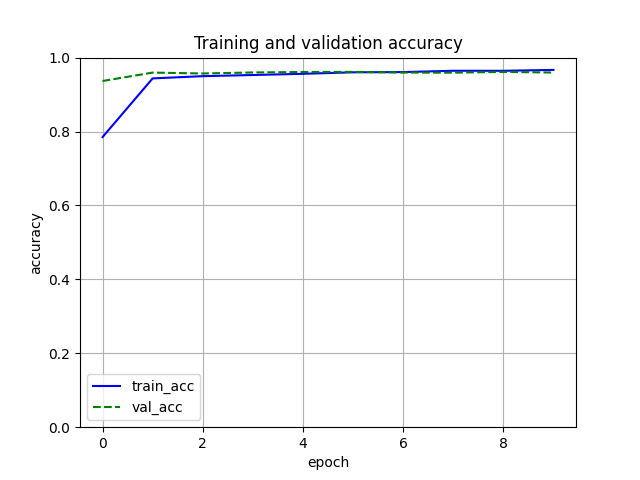
\includegraphics[width=\linewidth]{doushi_acc.png}
      \caption{動詞推定時の accuracy の推移}
      \label{fig:dou_acc}
\end{figure}
\begin{figure}[tbp]
      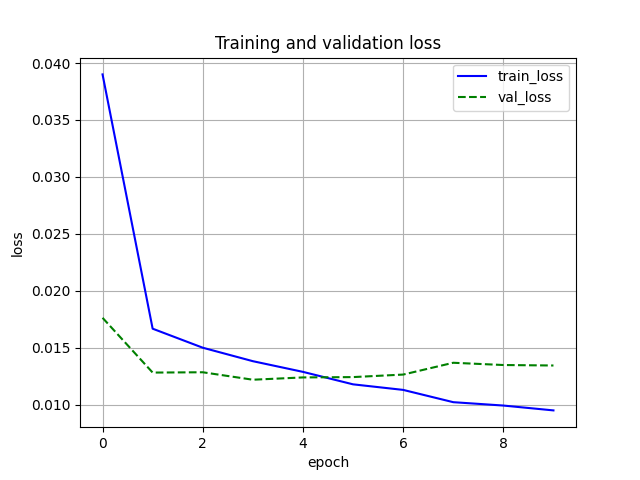
\includegraphics[width=\linewidth]{doushi_loss.png}
      \caption{動詞推定時の loss の推移}
      \label{fig:dou_loss}
\end{figure}

\begin{figure}[tbp]
      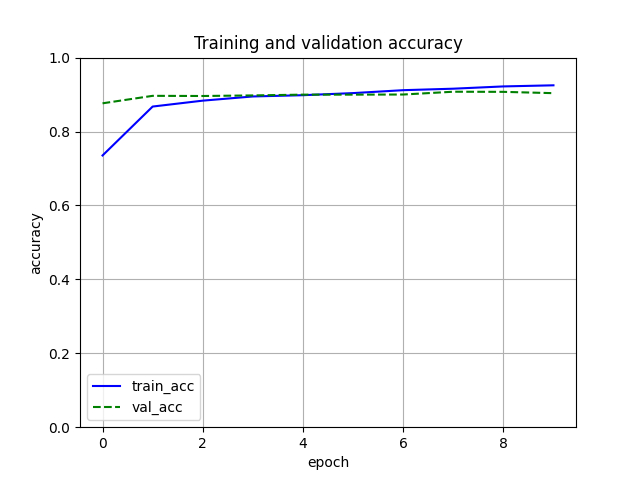
\includegraphics[width=\linewidth]{keiyoushi_acc.png}
      \caption{形容詞推定時の accuracy の推移}
      \label{fig:kei_acc}
\end{figure}
\begin{figure}[tbp]
      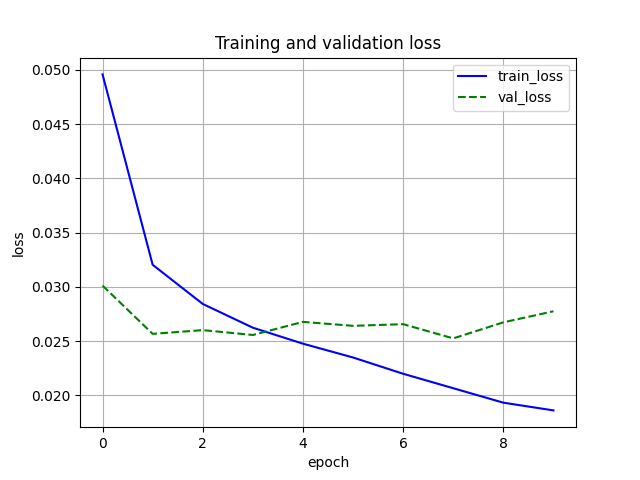
\includegraphics[width=\linewidth]{keiyoushi_loss.png}
      \caption{形容詞推定時の loss の推移}
      \label{fig:kei_loss}
\end{figure}



\begin{table}[t]
	\caption{実験精度}
	\begin{tabular}{| c |  c |} \hline
  品詞 & 平均値(標準偏差)  \\ \hline \hline
  名詞 & 0.914 (0.004) \\ %\cline{2-2}
  動詞 & 0.953 (0.004) \\
  形容詞 & 0.905 (0.004) \\
  ベースライン & 0.500 \\ \hline
	\end{tabular}
	\label{tb:2}
\end{table}





% 表 \ref{tb:2} にそれぞれのデータセットに対して 5 分割交差検証をした際の実験精度を示す.
%
%
% \begin{table}[t]
% \caption{実験精度}
%   \begin{tabular}{| c |  c | c |} \hline
%     品詞 & Accuracy & 平均値(標準誤差) \\ \hline \hline
%     		& 0.9017 &  \\ %\cline{2-2}
%     		& 0.9000 &  \\
%  名詞  	& 0.8900 & 0.8942 \\
%           & 0.8917 & (0.0056) \\
%        	& 0.8878 &  \\ \hline
% %
%               & 0.9539 &  \\ %\cline{2-2}
%        	& 0.9600 &  \\
%     動詞 	& 0.9533 & 0.9564 \\
%           & 0.9522 & (0.0042) \\
%        	& 0.9628 &  \\ \hline
% %
%               & a &  \\
%        	& a &  \\
%     形容詞 	& a &  \\
%           & a &  \\
%        	& a &  \\ \hline
% %
%     ベースライン & 0.5000 & 0.5000 \\  \hline
%   \end{tabular}
%   \label{tb:2}
% \end{table}





 \subsection{考察}
 実験の結果から,名詞,動詞,形容詞のいずれにおいても,高い精度で品詞の推定ができた.

\section{まとめと今後の課題}
本実験では,文中の単語がある品詞かそうでないかの 2 クラスに分類し,BERT を用いた推定精度を確認した.結果として,名詞,動詞,形容詞のいずれにおいても,高い精度で品詞を推定できることが分かった.このことから BERT は,隠された単語であってもその単語の品詞情報を獲得することができるため,適切な品詞の単語を補って文を生成することができると考えられる.\par
今後の課題としては以下のようなものが挙げられる.
\begin{itemize}
  \item BERT の出力で得られる単語の分散表現を用いた,単語の意味情報を取得できているかの確認
  \item 一文の複数箇所を "[MASK]" 記号に置き換えた場合にも品詞情報が正しく獲得できるかの確認
  % \item 上記のモデルの精度の向上
\end{itemize}





% 参考文献出力
\bibliography{index}
\bibliographystyle{unsrt}


\end{document}
